\subsection{Recognising Memoryless adversarially resolvable automata}\label{appendixsubsec:np-completeness}

\paragraph*{Token games}

For a parity automaton $\Ac$, the 2-token game on $\Ac$ is defined similarly to the HD game on $\Ac$ (\cref{defn:hd-game}), with Adam building a word letter-by-letter and Eve building a run on her token on Adam's word transition-by-transition, but additionally, Adam is also building two runs on two of his tokens transition-by-transition. The winning condition for Eve is that if any of the runs of Adam's tokens are accepting, then the run on her token is also accepting.

\begin{definition}\label{defn:twotokengame}
Given a nondeterministic parity automaton $\Ac=(Q,\Sigma,\Delta,q_0)$, the $2$-token game on $\Ac$ is a two-player non-stochastic complete-observation game between Eve and Adam that starts with an Eve's token and Adam's two distinguishable tokens at $q_0$, and proceeds in infinitely many rounds. In round $i$ when Eve's token is at $q_i$ and Adam's tokens are at $p^1_i$ and $p^2_i$:
\begin{enumerate}
    \item Adam selects a letter $a_i\in\Sigma$;
    \item Eve selects a transition $q_i\xrightarrow{a_i:c_i}q_{i+1}$ and moves her token to $q_{i+1}$;
    \item Adam selects transitions $p^1_i\xrightarrow{a_i:c^1_i}p^1_{i+1}$ and $p^2_i\xrightarrow{a_i:c^2_i}p^2_{i+1}$ on each of his tokens and moves his first and second token to $p^1_{i+1}$ and $p^2_{i+1}$, respectively.
\end{enumerate}
In the limit of a play of the $2$-token game, Eve constructs a run on her token, and Adam constructs a run on each of his two tokens, all on the same word. We say that Eve wins such a play if the run on her token is accepting or both the runs on Adam's tokens are rejecting. We say Eve \emph{wins the 2-token game} on $\Ac$ if she has a strategy to win the 2-token game.
\end{definition}

The rest of the section of the appendix will focus on the proof of \cref{lemma:ZlkDAGMDP}, which is restated below.
\ZlkDAGMDP*
\begin{proof}
        We begin by stating a lemma proved by Gimbert and Horn~\cite{GH10} for any prefix-independent objective---a property that Muller objectives satisfy.
        \begin{theorem}[\!\!\protect{\cite[Theorem~3.2]{GH10}}]\label{lemma:lastminute}\label{lemma:tailobjectives}
            If a player, say Adam, wins with a positive probability from some vertex of a complete-information two-player stochastic games, then he wins almost-surely from at least one vertex.
        \end{theorem}
        The following is a corollary of \cref{lemma:lastminute}, described in the work of Gimbert, Oualhadj, and Paul. 
        \begin{corollary}[\!\!\protect{\cite[Corollary~1]{GOP11}}]\label{cor:tailobjectives}
            If the set of vertices from which Adam wins almost-surely in an MDP with prefix-independent objectives can be computed in polynomial time, then there is also a polynomial time algorithm to compute the set of vertices from which Adam wins with positive probability. % what is exact value 
        \end{corollary}
       We note that the additional time taken to compute the vertices that wins with positive probability is, in fact, linear. 
        Because of \cref{cor:tailobjectives}, we will focus only on providing an $\Oh(|\Mc||\Zc_{C,\Fc}|)$-time algorithm to compute the almost-sure winning region for Adam. 
        
        Consider an MDP $\Mc$, with a Muller objective that is specified using a colouring function  $\col \colon E \rightarrow C$ over the edges of the MDP. 
        Let the Zielonka DAG representing the winning condition be $\Zc_{C,\Fc}$. Recall that vertices of the DAG are elements of the subset of colours, that is, if $\mu_X\in V(\Zc_{C,\Fc})$, then $X\subseteq C$. We can assume that the DAG $\Zc_{C,\Fc}$ has exactly one source node, $\nu_C$. The source node of a Zielonka DAG is either labelled by an accepting subset, that is, a subset  in $\Fc$, or by a rejecting subset, that is not in $\Fc$. %If the source node $\nu_X$ is accepting then all its successors $\nu_{Y_1},\dots,\nu_{Y_t}$ are all rejecting. If not and the label of the source node is rejecting, then its successors $\nu_{Y_1},\dots,\nu_{Y_t}$ are accepting. 
        \paragraph*{Maximal End Components} An end component
        of an MDP $\Mc = (V_A,V_R, E,\delta)$ is a subset of the vertices $V$ of the arena such that 
        \begin{itemize}
            \item the subgraph induced by $M$ in the graph $(V,E)$ is a strongly connected component, and
            \item for every $v\in V_R$ and for edges $v\rightarrow w\in E$, we have $w\in M$.
        \end{itemize}
        A Maximal End Component (MEC) is an end component that is maximal with respect to inclusion order. 
        
        Every vertex of an MDP belongs to at most one MEC. From every vertex in the MEC $M$, Adam can ensure that all vertices in $M$ are visited infinitely often, and the play starting from $M$ stays within $M$ with probability $1$. A MEC can be computed in polynomial time and even sub-quadratic time~\cite{CH11}.
        
        Consider the subroutine that takes as input an MDP $\Mc$ with a colouring function $\col$ from vertices $V$ to a finite set of colours $C$, along with a Zielonka DAG $\Zc_{C,\Fc}$ that uniquely represents the winning condition. 

        For a subset $X$ of colours, we write $\Mc|_X$ to denote the sub-MDP of $\Mc$ restricted to vertices in $\Mc$ from which the player Adam can ensure that all colours seen are within $X$ with probability $1$.  
        For an end-component $M$, we write $\col(M)$ to represent the set of all edge colours for all edges between two vertices in $M$. Therefore, $\col(M) = \{c\mid c= \col(u,v)\text{ and }u,v\in M\}$

        We refer to the reverse topological order of the nodes in a DAG to refer to the ordering $\nu_{X_1},\nu_{X_2},\dots,\nu_{X_d}$ of the nodes such that there is no edge $\nu_{X_i}\rightarrow\nu_{X_j}$, where $j<i$, that is, no node has an edge to a node occurring earlier than this in the order. 
        \begin{algorithm}
            \begin{algorithmic}\caption{A bottom up Zielonka-DAG algorithm to compute almost-sure winning sets in MDPs with Muller Objective}\label{algo:AlmostSureZielonkaDAG}
                \Procedure{AlmSureReach}{$\Mc, T$}
                    \State \Return{set of vertices in $\Mc$ from which player can almost surely reach $T$}
                \EndProcedure
                \Procedure{AlmostSureMuller}{$\Mc,\Dc$}
                        \For{nodes $\nu_X$ in reverse topological order in $\Zc_{C,\Fc}$}
                            \If{$X$ is an accepting set of colours}
                                \For{ $M_i\in M_1,\dots,M_k$, where each $M_i$ a maximal end components of $\Mc|_X$}
                                    \If{$\col(M_i)\cap \Bar{Y_j} \neq \emptyset$ for all $Y_j$ such that $\nu_X\rightarrow\nu_{Y_j}$}
                                    \State $\Win_{\nu_X}\gets\Win\cup M_i$
                                    \State $\Win\gets\textsc{AlmSureReach}_\Mc(\Win_{\nu_X})$
                                    \EndIf
                                \EndFor
                            \EndIf
                        \EndFor
                    \Return $\Win$
                \EndProcedure
            \end{algorithmic}
            \end{algorithm}
    \paragraph*{Correctness}
    We show that the procedure $\textsc{AlmostSureMuller}(\Mc,\Dc)$ returns exactly the set of vertices of the MDP from which Adam can satisfy the Muller objective with probability~$1$. 
    Let $W$ represent the set of vertices from which there is a strategy for Adam to ensure the Muller objective is satisfied with probability $1$. We show that $W = \Win$, where $\Win$ is the set returned by \cref{algo:AlmostSureZielonkaDAG}.  
    
    $W\subseteq\Win$. 
    We show that any vertex that is almost-surely winning is added to $\Win$ by \cref{algo:AlmostSureZielonkaDAG}. We say that an end components $M$ of the MDP is \emph{$\Fc$-winning} if $\col(M)$ is an accepting Muller set. 
    We use the following lemma to prove $W\subseteq\Win$.
    \begin{lemma}[\!\!\protect{\cite[Lemma~9]{Cha07}}]\label{lemma:Cha07Union}
        The vertices from which the player can achieve the Muller objectives with probability $1$ (the set of vertices $W$) are exactly the set of vertices that  can reach the union of all $\Fc$-winning end components with probability $1$.
    \end{lemma}
    % From this lemma, it is enough to show that 
    
    % \begin{claim}
    %     There is a strategy for Adam to win from all vertices of an $\Fc$-winning component $M$ almost-surely.
    % \end{claim} 
    % If there is a winning strategy for Adam, there is one where he uses no memory and only randomises between a few outgoing edges~\cite{CAH04}. Adam just follows his winning strategy that ensures that he visits all vertices in $M$ infinitely often without leaving. In fact, the following lemma says that all vertices that are winning are a union of such end components.
    From \cref{lemma:Cha07Union}, it is enough to show that for any end component $M$ such that all vertices almost-surely satisfies the Muller objective, $M\subseteq \Win$. Indeed, since $\Win$ that is returned by the algorithm is closed under almost-sure attractors, if all such $\Fc$-winning end components are in $\Win$, all almost-sure winning vertices are in $\Win$.
    
    Consider an end component $\Mc$ that is $\Fc$-winning. Then there is a node $\nu_X$ in the DAG that is the earliest (in reverse topological order) node such that $X$ is an accepting subset of colours and $X\supseteq \col(M)$ and $\col(M)\nsubseteq Y_j$ for any $\nu_{Y_j}$ that has an edge from $\nu_X$. Such a $\nu_X$ exists because $\col(M)$ is an accepting set, and since $\col(E)$ is the root of the DAG. The set would just be the smallest superset of $\col(M)$ among the labels of the nodes of the DAG. 
    
    In the sequel, we show the stronger statement that $\Fc$-winning end component $M$ satisfies $M\subseteq \Win_{\nu_X}$. 
    In $\Mc|_X$, the $\Fc$-winning $M$ is also an end component, since it contains winning vertices in $X$. Moreover, this end component $M$ is contained in some maximal end component $M_i$. Since $\col(M_i)\supseteq \col(M)$, and we assumed $\nu_X$ was the earliest node, it follows from the structure of the DAG that $X$ is a minimal subset of accepting colours containing $\col(M)$. Therefore, it must also be the case that $\col(M)\nsubseteq Y_i$ for any outgoing $\nu_{Y_i}$, such that $\col(M)\nsubseteq Y_i$. %, since otherwise $Y_i$ would be minimal
    Therefore, $M_i$, which is a superset of $M$, is added to $\Win_{\nu_X}$, and therefore $\Win$.
    
   % Therefore, when the algorithm terminates, all end components that that satisfies the Muller objective are in $\Win$. Since the algorithm returns the set of vertices that is almost sure reachable to such a set $\Win$, we can conclude that the almost sure winning set $W\subseteq \Win$.

    \textit{$\Win\subseteq W$.} We provide a winning strategy for every vertex in $W$ that almost-surely achieves the Muller objective.  Since $\Win$ is monotonically increasing, that is, vertices are added and not removed, we consider the first time that a vertex $v$ was added.

    We argue that the algorithm maintains the invariance that from any vertex in $\Win$, there is a strategy such that the Muller objective is satisfied with probability $1$ using a strategy that only visits the vertices in $\Win$.  Trivially this is true when $\Win = \emptyset$. 

    When a vertex $v$ is added to the set, it is because either $v\in M_i$ for some MEC of $\Mc|_X$ or because $v$ is almost surely reachable to $\Win_{\nu_X}$.
    If it was the former, then consider the strategy of the player that visits all vertices in $M_i$ infinitely often, while avoiding all vertices whose colour is not in $X$.  Such a strategy exists since $\Mc|_X$ is defined as the sub MDP from which the player could avoid any colour not in $X$, and further $M_i$ is a maximal end component ensuring that by randomising between all the edges in $M_i$, the set of colours seen infinitely often is exactly $\col(M_i)$ which is a winning subset of colours. 
    If the vertex $v$ was added because it had an almost sure reachability strategy to $\Win$, then from $v$, the player follows that strategy to reach the set $\Win_{\nu_X}$, and later follows the existing winning strategy for vertices defined for the vertices $\Win_{\nu_X}\subseteq \Win$. 
    \paragraph*{Runtime} The algorithm runs in time that is polynomial in the size $m$ of the MDP and the size $d$ of the DAG $\Zc_{C,\Fc}$. More precisely, we show that the runtime is at most $\Oh( m\cdot d)$.
    This is because topologically sorting the nodes of the DAG $\Dc$ takes time at most $\Oh(d)$ using Tarjan's algorithm~\cite{Tar72}. 
    Later, for each node $\nu_X$, the algorithm computes an MDP that avoids colours not in $X$, and then computes the maximal end components of such MDPs. This step takes time that is linear in the size of the MDP~\cite{CH11}. Finally, computing the almost sure reachable set of vertices can also be done in linear time in the number of states in the MDP. Therefore, the time taken is at most $\Oh(m\cdot d)$
\end{proof}
\MAcheckNPhard*
\begin{proof}
    We will use the proof by Prakash that showed NP-hardness for the problem of deciding history-determinism~\cite{Pra24a}. There, the reduction is from the problem of solving \emph{good 2-D parity games}, which we define first. 

    A \emph{2-dimensional parity game} $\Gc$ is a complete-observation non-stochastic game, where each edge $e = (u,v)$ in $\Gc$ is labelled with two priorities $(f_e,s_e)$. We call $f_e$ and $s_e$ as the first and second priority of $e$, respectively and write the edge $e$ as $e=u\xrightarrow{f_e,s_e}v$. We say that an infinite play in $\Gc$ satisfies the first (resp.\ second) parity condition if the largest first (resp.\ second) priority occurring infinitely often amongst the edges of that play is even. An infinite play $\rho$ in $\Gc$ is winning for Eve if the following condition holds: \emph{if $\rho$ satisfies the first parity condition, then $\rho$ also satisfies the second parity condition}. Otherwise, Adam wins that play. We say Eve wins $\Gc$ if she has a sure winning strategy, i.e., any play constructed when Eve is playing according to that strategy is winning.

    We say that a 2-dimensional parity game $\Gc$ is \emph{good} if all plays that satisfy the first parity condition also satisfy the second parity condition. The problem of deciding if Eve wins good 2-D parity games is $\NP$-complete~\cite[Lemma 13]{Pra24a}.  

    We reduce the problem of deciding if Eve wins a good 2-D parity game to deciding if a parity automaton is MA, by showing that the reduction of \cite{Pra24a}, starting from a good 2-D parity game $\Gc$, constructs $\Hc$, such that $\Hc$ contains a deterministic subautomaton $\Dc$ and:
    \begin{enumerate}
        \item if Eve wins $\Gc$, then $\Hc$ simulates $\Dc$ and $\Hc$ is determinisable-by-pruning, and therefore, $\Hc$ is MA.
        \item if Adam wins $\Gc$, then $\Hc$ does not simulate $\Dc$, $\Hc$ is not HD, and hence $\Hc$ is not MA.
    \end{enumerate}
    \paragraph*{The reduction}
    Let $\Gc$ be a 2-D parity game. We next describe the construction of $\Hc$ as above. The automata $\Hc$ will contain a deterministic subautomaton $\Dc$ and is over the alphabet $\Sigma = E\cup \$$. Informally, the priorities of transitions of $\Dc$ and $\Hc$ will capture the first and second priorities of edges in $\Gc$, respectively. 
    
    For each Adam vertex $v$, we have the states $v_D$ in $\Dc$ and $v_H$ in $\Hc$. For each edge $e = v\xrightarrow{f_e:s_e} u$ outgoing from $v$, we have the transitions $v_D \xrightarrow{e:f_e} u_{\$}$ and $v_H \xrightarrow{e:s_e} u_H$ on the letter $e$ (see \cref{fig:Adam-vertex}).
    
% \begin{figure}[!htb]
%     \centering
%     \begin{minipage}{0.4\linewidth}
      %\begin{figure}
       %\centering

    %\end{figure}  
  %   \end{minipage}\hfill\hfill
  % \begin{minipage}{0.6\textwidth}

    Adam choosing an outgoing edge from $v$ in $\Gc$ is captured by a round of the simulation game where Adam's token is in $v_D$ and Eve's token is in $v_H$. This way, Adam, by choice of his letter in the simulation game, captures the choice of outgoing edges from his vertex. 
       \begin{figure}
           \centering
    \begin{subfigure}[b]{0.45\linewidth}
    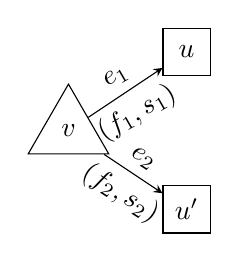
\begin{tikzpicture}
        \usetikzlibrary{graphs,quotes}
        \usetikzlibrary{backgrounds,scopes,fit,shapes.geometric}
         \node (v) [regular polygon, regular polygon sides = 3, minimum size = 0.25 cm, draw]    at (0,0)   {$v$};
         \node (u1) [rectangle, minimum size = 0.6 cm, draw] at (1.5,1) {$u$};
         \node (u2) [rectangle, minimum size = 0.6 cm, draw] at (1.5,-1) {$u'$};
         \path[-stealth]
         (v) edge node [above, rotate = 30] {$e_1$} node [below, rotate = 30] {$(f_1,s_1)$} (u1)
         (v) edge node [above, rotate = 327] {$e_2$} node [below, rotate = 327] {$(f_2,s_2)$} (u2)
         ;
    \end{tikzpicture}
    \caption{An Adam vertex (drawn as a triangle) and its outgoing edges in $\Gc$}\label{fig:Adam-vertexa}
    \end{subfigure}~
    \begin{subfigure}[t]{0.5\linewidth}
    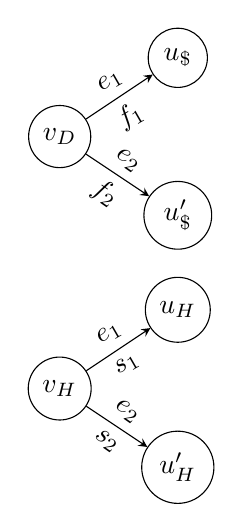
\begin{tikzpicture}
        \usetikzlibrary{graphs,quotes}
        \usetikzlibrary{backgrounds,scopes,fit,shapes.geometric}    
        \node (vD) [circle, minimum size = 0.5 cm, draw] at (0,0) {$v_D$};
         \node (u1dollar) [circle, minimum size = 0.5 cm, draw] at (1.5,1) {$u_\$$};
         \node (u2dollar) [circle, minimum size = 0.5 cm, draw] at (1.5,-1) {$u'_{\$}$};
    
         \node (vH) [circle, minimum size = 0.5 cm, draw] at (0,-3.2) {$v_H$};
         \node (u1H) [circle, minimum size = 0.5cm, draw] at (1.5,-2.2) {$u_H$};
         \node (u2H) [circle, minimum size = 0.5cm, draw] at (1.5,-4.2) {$u'_H$};
    
    
         \path[-stealth]
         (vD) edge node [above, rotate = 30] {$e_1$}  node [below, rotate = 30] {$f_1$} (u1dollar)
         (vD) edge node [above, rotate = 325] {$e_2$} node [below, rotate = 325] {$f_2$} (u2dollar)
         (vH) edge node [above, rotate = 30] {$e_1$} node [below, rotate = 30] {$s_1$} (u1H)
         (vH) edge node [above, rotate = 325] {$e_2$} node [below, rotate = 325] {$s_2$} (u2H)
        ;
    \end{tikzpicture}
    \caption{Corresponding states and transition in $\Hc$ and $\Dc$.}\label{fig:Adam-vertexb}
    \end{subfigure}
    \caption{Transitions corresponding to Adam's vertices. The letters are displayed on top, and the priorities are below each edge.}\label{fig:Adam-vertex}
    \end{figure}
    For each Eve vertex $v$ and outgoing edge $e = v\xrightarrow{f,s}u$ from that vertex, we will have the states $v_{\$}$, $v_D$, and $u_D$ in $\Dc$, and the states $v_H$, $(v_H,e)$, and $(u_H)$ in $\Hc$. In $\Dc$, we will have the transitions $v_\$ \xrightarrow{\$:0} v_D, v_D \xrightarrow{e:f}: (u_D)$, and in $\Hc$, we will have the transitions $v_H \xrightarrow{\$:0} (v_H,e), (v_H,e) \xrightarrow{e:s} u_H$. Additionally, for every outgoing edge $e'=v\xrightarrow{f',s'}u'$ that is different from $e$, we add the transition $(v_H,e) \xrightarrow{e':s'} u'_D$ (see \cref{fig:Eve-vertex}).  
      \begin{figure}
      \centering
\begin{subfigure}[b]{0.35\linewidth}
    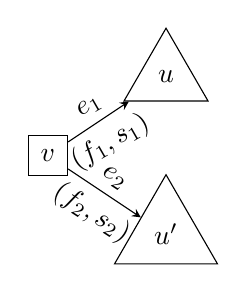
\begin{tikzpicture}
    \usetikzlibrary{graphs,quotes}
    \usetikzlibrary{backgrounds,scopes,fit,shapes.geometric}
    \node (v) [rectangle, minimum size = 0.5 cm, draw] at (0,0) {$v$};
     \node (u1) [regular polygon, regular polygon sides = 3, minimum size =0.3cm, draw]    at (1.5,1)   {$u$};
     \node (u2) [regular polygon, regular polygon sides = 3, minimum size = 0.3cm, draw] at (1.5,-1) {$u'$};
      \path[-stealth]
     (v) edge node [above, rotate = 30] {$e_1$} node [below, rotate = 30] {$(f_1,s_1)$} (u1)
     (v) edge node [above, rotate = 327] {$e_2$} node [below, rotate = 327] {$(f_2,s_2)$} (u2)
     ;
    \end{tikzpicture}
    \caption{An Eve vertex (drawn as a square) and its outgoing edges in $\Gc$}\label{fig:Eve-vertexa}
\end{subfigure}~
\begin{subfigure}[t]{0.57\linewidth}
    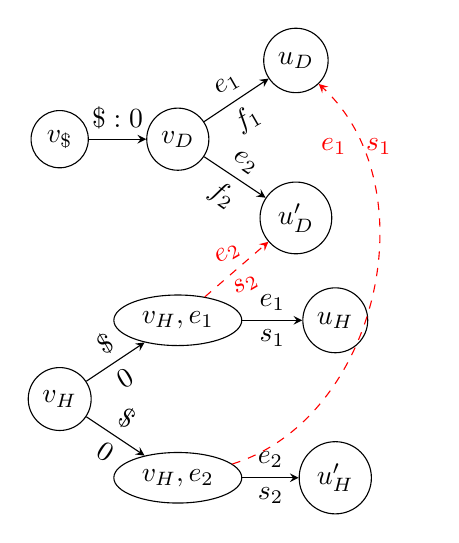
\begin{tikzpicture}
        \usetikzlibrary{graphs,quotes}
    \usetikzlibrary{backgrounds,scopes,fit,shapes.geometric}
     \node (vdollar) [circle, minimum size = 0.5 cm, draw] at (0,0) {$v_\$$};
     \node (vD) [circle, minimum size = 0.5 cm, draw] at (1.5,0) {$v_D$};
     \node (u1D) [circle, minimum size = 0.5 cm, draw] at (3,1) {$u_D$};
    \node (u2D) [circle, minimum size = 0.5 cm, draw] at (3,-1) {$u'_D$};     

     \node (vH) [circle, minimum size = 0.5 cm, draw] at (0,-3.3) {$v_H$};
     \node (e1) [ellipse, minimum size = 0.5cm, draw] at (1.5,-2.3) {$v_H,e_1$};
     \node (e2) [ellipse, minimum size = 0.5cm, draw] at (1.5,-4.3) {$v_H,e_2$};
     \node (u1H) [circle, minimum size = 0.5 cm, draw] at (3.5,-2.3) {$u_H$};
     \node (u2H) [circle, minimum size = 0.5 cm, draw] at (3.5,-4.3) {$u'_H$};
    
     \path[-stealth]
     (vdollar) edge node [above] {$\$:0$} (vD)
     (vH) edge node [above, rotate = 30] {$\$$} node [below, rotate = 30] {$0$} (e1)
    (vH) edge node [above, rotate = 327] {$\$$} node [below, rotate = 327] {$0$} (e2) 
     
     (vD) edge node [above, rotate = 30] {$e_1$}  node [below, rotate = 30] {$f_1$} (u1D)
     (vD) edge node [above, rotate = 325] {$e_2$} node [below, rotate = 325] {$f_2$} (u2D)
    
    (e1) edge node [above] {$e_1$} node [below] {$s_1$} (u1H)
     (e2) edge node [above] {$e_2$} node [below] {$s_2$} (u2H)

    
    (e1) edge [red, dashed] node [above, rotate = 30] {$e_2$} node [below, rotate = 30] {$s_2$} (u2D)
    (e2) edge [red, dashed, bend right = 60] node [left,yshift=19mm,xshift=-2mm] {$e_1$} node [right,yshift=19mm,xshift=-2mm] {$s_1$} (u1D)
    ;
\end{tikzpicture}
\caption{Corresponding states and transition in $\Hc$ and $\Dc$.}\label{fig:Eve-vertexb}
\end{subfigure}    
\caption{Transitions corresponding to Eve's vertices. The letters are displayed on top, and the priorities are below each edge}\label{fig:Eve-vertex}
\end{figure}

    
    Eve's choosing of an outgoing edge from $v$ in $\Gc$ is captured by two rounds of the simulation game where at the start, Adam's token is in $v_{\$}$ while Eve's token is in $v_H$. Then, Adam selects the letter $\$$ and his token takes the transition to $v_D$. Then Eve can move her token to any state of the form $(v_H,e)$, where $e$ is an outgoing edge from $v$ in $\Gc$. Thus, Eve, by choice of her transition on $\$$ from $v_H$, captures the choice of outgoing edges available from her vertex. When Adam's token is at the state $v_D$ and Eve's token is at the state $(v_H,e)$, Adam can either replay the edge $e$ as the next letter, from where Adam's token goes to $u_H$ and $v_H$. Or, Adam can choose another edge $e'=(v,u')$ that is outgoing from $v$ as the letter: this causes both Eve's and Adam's token to be in the same state $u'_D$, from where Eve trivially wins the simulation game. We call these moves of Adam as \emph{corrupted moves}, and they cause Eve's token to take the dashed transitions in~\cref{fig:Eve-vertex}. 

    We suppose that the initial state of $\Gc$ is an Adam vertex $v$, and we let the initial state of $\Hc$ and $\Dc$ be $v_H$ and $v_D$, respectively. This concludes our description of $\Hc$ and $\Dc$.

    \paragraph*{Correctness of the reduction}
    Note that any play of the simulation game of $\Dc$ by $\Hc$ where Adam does not take any corrupted moves will correspond to a play of the game $\Gc$. The priorities of Adam's token and Eve's token corresponds to the first and second priorities of the edges in $\Gc$, respectively. Thus, Eve wins $\Gc$ if and only if $\Hc$ simulates $\Dc$. For a more rigorous proof, we refer the reader to \cite{Pra24a}.  

   Note that since $\Gc$ is good, any play satisfies the first parity condition also satisfies the second parity condition: this implies that $\Lc(\Dc) \subseteq \Lc(\Hc)$. Since $\Dc$ is a subautomaton of $\Hc$, we obtain that $\Lc(\Dc) = \Lc(\Hc)$. Thus, $\Hc$ simulates $\Dc$ if and only if $\Hc$ is HD if and only if Eve wins $\Gc$ (\cref{lemma:hd-equiv-detsimulation}). 
   
   If Eve wins a 2-dimensional parity game, then Eve has a positional pure winning strategy~\cite[Page 158]{CHP07}. Thus, if Eve wins $\Gc$, then she has a positional strategy given by $\sigma:V_{\eve} \xrightarrow{} E$. This yields a positional strategy for Eve in the HD game on $\Hc$, where from the vertex $v_H$ for $v \in V_{\eve}$ and on the letter $\$$, she chooses the transition  to $(v_H,(v_H,\sigma(v_H)))$. Thus, $\Hc$ is determinisable-by-pruning and hence MA.

   Otherwise, if Eve loses $\Gc$, then $\Hc$ is not HD and hence not MA. This shows the correctness of the above reduction. Thus, the problem of deciding if an automaton is MA is NP-hard.
\end{proof}

\subsection{Recognising SR and MA automata and verifying resolvers}

\lemmaUndecidablecoBuchi*
\begin{proof}
We reduce from the problem of checking the emptiness of a B\"uchi probabilistic automata under the probabilistic semantics.

\begin{question}[\textsf{PBA-Emptiness}]
    Given a probabilistic B\"uchi automaton, is there a word $w$ on which the probability of a run being accepting is non-zero?
\end{question}


\paragraph*{Construction}
Consider a probabilistic B\"uchi automaton $\Bc = (Q_\Bc,\Sigma,\Delta_\Bc,s)$ over the alphabet $\Sigma$. We will construct a non-deterministic coB\"uchi automaton $\Cc$ similar to the one in \cref{fig:ReductioncoBuchi}. We give a formal definition of $\Cc = (Q_\Cc,\Sigma', \Delta_\Cc,s)$ below where the
\begin{itemize}
    \item alphabet is $\Sigma' = \Sigma\cup \{\$,a,b\}$,
    \item states $Q_\Cc = Q_\Bc\uplus \{s, s_1, s_2, s_{\text{fin}}\}$,
    \item initial state is $s$
    \item transitions are $\Delta_{\Cc} = \Delta_{\Bc}' \uplus\{
    s\xrightarrow{\$: 0}s_1,
    s\xrightarrow{\$: 0}s_2,
    s_1\xrightarrow{a: 0}q_0,
    s_2\xrightarrow{b: 0}q_0, 
    s_1\xrightarrow{b: 0}s_{\text{fin}}, 
    s_2\xrightarrow{b: 0}s_{\text{fin}}\} $ where $\Delta_{\Bc}' = \{q \xrightarrow{a:0}q'\mid q \xrightarrow{a:1}q'\in \Delta_{\Bc} \}\cup \{q \xrightarrow{a:1}q'\mid q \xrightarrow{a:2}q'\in \Delta_{\Bc} \}$.
\end{itemize}
Consider the following memoryless (finite memory) resolver $\Rc$ which outputs with probability $1/2$ one of the two transitions $s\xrightarrow{\$: 0}s_1$ and $s\xrightarrow{\$: 0}s_2$ out of the initial state $s$. 
The memoryless resolver further outputs transitions with the exact probability distributions as the probabilistic automaton $\Bc$ from all the states in $Q_\Bc$. At states $s_1,s_2,s_{\text{fin}}$ from where the transitions are deterministic, the resolver chooses the unique transition available on that letter with probability $1$. 
\begin{figure}
    \centering
    \begin{tikzpicture}[shorten >=1pt, node distance=1.5cm, on grid, auto]
     \tikzstyle{state}=[circle, draw, minimum size=15pt, inner sep=1pt]
  % States
  \node[state, initial,initial text=] (q0) {$s$};
  \node[state] (q1) [above right=of q0] {$s_1$};
  \node[state] (q2) [below right=of q0] {$s_2$};
  \node[state] (q3) [right=of q1] {$q_0$};
  \node[state] (q4) [right=of q2] {$s_\textsf{fin}$};

  % Edges
  \path[->]
    (q0) edge node[sloped]  {$\$\colon \frac{1}{2}$} (q1)
    (q0) edge node[sloped,swap]  {$\$\colon \frac{1}{2}$} (q2) 
    (q1) edge node[sloped] {$a$} (q3)
    (q1) edge node[above, xshift=-3mm, yshift = 4mm] {$b$} (q4)
    (q2) edge node[sloped,swap] {$a$} (q4)
    (q2) edge node[below , xshift=-3mm, yshift = -4mm] {$b$} (q3)
    (q4) edge[loop right] node{$\Sigma$} (q4);

    \draw (2,0) rectangle (4.5,1.5);
      \node (q1) at (3.5,0.7) {$\Bar{\mathcal{B}}$};
\end{tikzpicture}
    \caption{Constructing a coB\"uchi $\Cc$ automaton where $\Bar{\Bc}$ is the dual of the probabilistic B\"uchi automaton $\Bc$}
    \label{fig:ReductioncoBuchi}
\end{figure}


% \begin{figure}[h]
%     \centering
%     \includegraphics[scale=0.4]{ReductioncoBuchiResolver.png}
%     \caption{A reduction constructing a resolver for a coB\"uchi automaton where $\Bar{\Bc}$ is the dual of the probabilistic B\"uchi automaton $\Bc$ {\color{red}(replace $\Ac$ with $\Bc$ in the picture)}}
%     \label{fig:ReductioncoBuchi}
% \end{figure}

We will now show that the probabilistic automaton $\Bc$ accepts a word  $w\in \Sigma^\omega$ with probability $>0$ if and only if 
%there is some word $w\in \Sigma^\omega$ such that the probability of the run of $w$ on $\Bc$ that has an accepting run is $0$ if and only if
$\Rc$ is not an almost-sure resolver. 

\paragraph*{$\implies$} Suppose the PBA $\Bc$ accepts a word $w$ with probability $p>0$. 
Consider the word $ \$ a w$. On this word, the probability of the word being accepted is 
\begin{equation*} %\label{eq1}
\begin{split}
&\Pr[\text{reaching }s_1\text{ on } \$]\cdot \Pr[\Rc\text{ resolving } aw \text{ from }s_1] \\
        +  
    &\Pr[\text{reaching }s_2\text{ on } \$] \cdot \Pr[\Rc\text{ resolving } aw \text{ from }s_2] \\
    &= \frac{1}{2}\cdot\Pr[\Rc\text{ resolving } w \text{ from }q_0]\\
    &+ \frac{1}{2}\cdot\Pr[\Rc\text{ resolving } w \text{ from }s_{\text{fin}}]
\end{split}
\end{equation*}
From our construction, the resolver is such that the probability of $w$ having an accepting run from $q_0$ is $1-p$. Therefore, on $w$, the probability of acceptance by the resolver is $$\frac{1}{2} + \frac{1-p}{2} = 1-\frac{p}{2}<1.$$
\paragraph*{$\impliedby$} 
Suppose the resolver is \emph{not} an almost-sure resolver. This implies that there is a word $w$ in the language of the automaton $\Bc$ for which the probability of the run produced by a resolver is $p'<1$. Since the language is $\$(a+b)\Sigma^\omega$, the first two letters of the word should be $\$$ followed by $a$ or $b$. Without loss of generality, we assume the word is $\$aw$. 
The probability of a run chosen according to the resolver ends in state $q_0$ after reading $\$ a$ is $\frac{1}{2}$, and the probability that the run ends at state $s_{\text{fin}}$ after $\$ a$ is $\frac{1}{2}$. Let the probability of the resolver resulting in an accepting run from $q_0$ be $p$. Since all words in $\Sigma^\omega$ are accepting from $s_{\text{fin}}$, it must be that the probability $p'$ of the resolver producing an accepting run on $\$aw$ is $$\frac{p}{2} + \frac{1}{2} = \frac{1+p}{2}.$$
Since $p'<1$, we know $1+\frac{p}{2}<1$ and therefore $p<1$. Observe that from our construction, the probability $1-p$ is also the probability of the probabilistic B\"uchi automaton $\Bc$ accepting the word $w$. Therefore, there is a word $w$, such that the probability that $w$ is accepted with probability $1-p$, which is positive. 
\end{proof}
\lemmaUndecidableBuchi*

To prove \cref{lemma:UndecidableBuchi}, we will use an undecidability result from probabilistic automaton over finite words. A probabilistic finite automaton, or PFA for short, has similar syntax to an NFA, except that each transition is assigned a probability $0<p<1$, such that for each state and letter, the sum of probabilities of outgoing transitions from that state on that letter is $1$. The semantics of how runs work in PFA can be defined similarly to how we defined for probabilistic parity automata in \cref{sec:prelims}. We represent a PFA by a tuple $\Pc=(Q,\Sigma,\Delta,F,\rho,q_0)$, where $Q$ is the set of states, $\Sigma$ is the alphabet, $\Delta \subseteq Q \times \Sigma \times Q$ is the set of transitions, $F$ is the set of accepting states,  $\rho:\Delta \xrightarrow{} \unitinterval$ is the probability function, and $q_0$ is the initial state.

For a PFA $\Pc$ and a finite word $u$, we denote the probability that a random run of $\Pc$ on $u$ is accepting by $\prob_\Pc (u)$. 

\begin{proof}[Proof of \cref{lemma:UndecidableBuchi}]
As mentioned, we reduce from the zero-isolation problem.

\begin{question}[Zero-Isolation Problem] 
    Given a probabilistic automaton  $\Pc$ over finite words, is there a value $c>0$ such that for all words, the if the word has a non-zero probability of acceptance, then it is accepted by $\Pc$ with probability larger than $c$, that is, for all $w\in\Sigma^*$, is it true that $\prob_\Pc(w) =0 $ or $\prob_\Pc(w) > c$.
\end{question}   
The zero-isolation problem is undecidable~\cite[Theorem 4]{GO10}. 
We detail the reduction of the construction below and later prove the correctness afterwards. 
\paragraph*{Construction}
Let $\Pc$ be an PFA. We will construct a B\"uchi automaton $\Bc$ and a resolver $\Rc$ for $\Bc$ such that $\Rc$ is an almost-sure resolver of $\Bc$ if and only if $\Pc$ isolates zero. 

Let the set of all words accepted by $\Pc$ with non-zero probability be written as $\Lc_{>0}(\Pc)$. We will construct a B\"uchi automaton that accepts the language $\Lc_{>0}(\Pc)$ repeated with a symbol $\$$ as a separator between  two words from the language $\Lc_{>0}(\Pc)$, that is,  $$\Lc(\Bc) = \{w_1\$w_2\$\dots \$w_k\$\dots \mid w_i\in L_{>0}(\Pc)\}.$$
%We assume that $\Pc$ is complete, that is, for every word, the probability of the word having a run is $1$. If the automaton is not complete, then we can complete it by adding a sink state. 
We will construct $\Bc$ with the same set of states as the finite probabilistic automaton $\Pc$. 
The transitions of $\Bc$ are exactly the transitions from the probabilistic automata $\Pc$, where any probabilistic transition with non-zero probability are made into non-deterministic choices for $\Bc$. 
Finally, we add more transitions from all states of $\Pc$ to the starting state $q_0$ of $\Pc$ on the letter $\$$.
We need to assign priorities to the transitions of $\Bc$ to complete our construction of $\Bc$. We assign priority $2$ to the transitions on the letter $\$$ that go from a final state of $\Pc$ to $q_0$. We assign a priority of $1$ to all other transitions on $\Bc$.
The resolver $\Rc$ is a memoryless resolver that at state $q$ on letter $a$ uses the same probability distribution as dictated by the transition from $q$ on $a$ in $\Pc$.

Let $\Pc = \tpl{Q,\Sigma,\Delta,\rho,q_0}$. We construct a B\"uchi automaton $\Bc = (Q,\Sigma\uplus\{\$\},\Delta',q_0)$, where $\Delta' = \{q\xrightarrow{\$:1}q_0\mid q\notin F\}\cup \{q\xrightarrow{\$:2}q_0\mid q\in F\} \cup  \{q\xrightarrow{a:1}q_0\mid q\xrightarrow{a(p)}q_0\in\Delta, p>0\}$. An illustration is provided in \cref{fig:PBAfromPFA}. 
\begin{figure}
    \centering
    \begin{tikzpicture}[shorten >=1pt, node distance=2cm, on grid, auto]
   \node[state, initial, initial text=] (q_0) {$q_0$};
   \node[state, accepting, right=of q_0] (q_1) {$q_{f}^1$};
   \node[state, accepting, below=of q_1] (q_2) {$q_f^t$};
   \node[state, below=of q_0, yshift =6mm] (q_3) {$q_2$};
   \node (q_4) at (2.2,1)  {$F$};

   \path[->]
    (q_1) edge [bend right=70,double] node [above] {$\$$} (q_0)
    (q_2) edge [bend right=10, double] node [above] {$\$$} (q_0)
    (q_3) edge [bend left=30] node [left] {$\$$} (q_0);
    
   \draw[thick, rounded corners] 
        ($(q_0.north west)+(-0.3,0.3)$) rectangle ($(q_2.south east)+(0.2,-0.3)$);
 
   \draw[dashed] 
        ($(q_0.north east)+(1,0.3)$) -- ($(q_0.south east)+(1,-2.3)$);
\end{tikzpicture}
    \caption{Converting PFA $\Pc$ to a B\"uchi automaton $\Bc$ by adding transitions on $\$$. Other transitions in $\Bc$ include all transitions of $\Pc$ that have non-zero probability. }
    \label{fig:PBAfromPFA}
\end{figure}
Further, consider the resolver $\Rc$ that chooses the non-deterministic transitions $q\xrightarrow{\$:1}q_0$ with probability $\rho(q\xrightarrow{a}q_0)$ that is the same as the probability assigned to the transition by the automaton $\Pc$. Observe that language of $\Bc$ is words of the word $w_1 \$ w_2 \$ w_3 \$ \dots$, where each $w_i \in \Sigma^{*}$ and infinitely many $w_i$ are in $L_{>0}(\Pc)$.

$$\Lc(\Bc) = ( (\Sigma^{*} \$) (\Lc_{>0} (\Pc))\$ )^{\omega}.$$

We show that the resolver $\Rc$ is an almost-sure resolver  if and only if there is a value $c$ such that $\prob_\Pc(w)>c$ for all words $w$. 
% \begin{claimproof}
% Consider any word in $((\Sigma^*\$)^*R\cdot\$)^\omega$, we show that it has an accepting run in $\Bc$.
% Consider $\Bc$. The only accepting transition are of the form $q\xrightarrow{\$:2}q_0$, where $q$ is a final state of the PFA $\Pc$. 
% Any word that has an accepting run must have a run that starts at 
% \end{claimproof}
\paragraph*{$\implies$} Suppose $\Pc$ is a probabilistic automaton that does not isolate $0$. Then, for all  $n\in\Nb$ there is a finite word $w_n$, such that $0<\prob_\Pc(w_n)<1/{2^n}$. Consider the infinite word $w_1\$w_2\$w_3\$\dots\$ w_n\$\dots$. This word is in $\Lc(\Bc)$. However, we argue that the resolver $\Rc$ only produces an accepting run with probability $0$. Indeed, the probability of the resolver visiting a transition with priority 2 on the segment of the word $w_i\$$ is exactly the same as the probability of acceptance of $w_i$ in $\Pc$, which is a value between $0$ and $1/2^n$. 
Observe that $\sum_i^\infty \prob_\Pc(w_i)<\sum_i 1/{2^i} < 1$.
By the Borel-Cantelli lemma (\cref{lemma:borellcantelli}), if the infinite sum of the probabilities of events over an infinite sequence of events is finite, then the probability that infinitely many of the events occur is $0$. Therefore, the probability of a run on the word $w_1\$w_2\$w_3\$\dots\$ w_n\$\dots$ containing infinitely many accepting transitions is $0$.
\paragraph*{$\impliedby$}
Suppose $\Pc$ is a probabilistic automaton that isolates $0$, that is, there is a $c>0$, such that for all $w\in\Sigma^*$, either $\prob_\Ac(w) =0 $ or $\prob_\Ac(w) > c$. 
Consider any word in the language of $\Bc$ which is  $((\Sigma^*\$)^*R\cdot\$)^\omega$. This implies it consists of infinitely many substrings (disjoint) of the form $\$w_i\$$ where $\prob_\Pc(w_i) > 0$. Since $\Pc$ has an isolated $0$, we can further claim that $\prob_\Pc(w_i) > c$. Therefore for each $i$, the probability a run resolved using resolver $\Rc$ visiting an accepting state on reading $\$w_i\$$ is at least $c$. From the second Borel-Cantelli lemma (\cref{lemma:secondborellcantelli}), we know if the sum of probabilities of an infinite sequence of independent events is infinite, then the probability of infinitely many of the events occurring is $1$.
For each $i$, the events $E_i$ where the run obtained from the resolver $\Rc$ on reading $w_i$ contains an accepting transition are all independent events. 
Furthermore, the probability of each event $E_i$ is $\prob_\Pc(w_i)$ and since $\sum_i \prob_\Pc(w_i) > \infty$, we can conclude that the resolver produces an accepting run with probability $1$.
\end{proof}


